\documentclass{beamer}
\usepackage[style=verbose, backend=bibtex]{biblatex}
\usepackage{xcolor}
\usepackage{hyperref}

\addbibresource{adlproj.bib}

\usetheme{Madrid}
\usecolortheme{beaver}

\hypersetup{colorlinks=true,citecolor=blue, urlcolor=blue, linkcolor=blue,breaklinks=true}

\definecolor{darkred}{rgb}{0.8,0,0}
%Information to be included in the title page:
\title[Live Style Transfer] %optional
{Live Style Transfer}
\author{{\small Guillaume Bril - Hubert de Lesquen - Matthieu Denis - Alexandre Gommez}}
\institute{IPP - M2DS}
\date{30 mars 2022}
\subtitle{Applied Deep Learning Project}

%\setbeamercolor{section in toc}{fg=red}
%\setbeamertemplate{itemize item}[square]
\setbeamercolor{itemize item}{fg=darkred}
\setbeamertemplate{itemize item}[default]

%\setbeameroption{show notes}
%\setbeameroption{show only notes}
%\setbeameroption{show notes on second screen=right}

\makeatletter
\setbeamertemplate{footline}{
  \leavevmode%
  \hbox{%
  \begin{beamercolorbox}[wd=.4\paperwidth,ht=2.25ex,dp=1ex,center]{institute in head/foot}%
    \usebeamerfont{institute in head/foot}\insertshortinstitute
  \end{beamercolorbox}%
  \begin{beamercolorbox}[wd=.3\paperwidth,ht=2.25ex,dp=1ex,center]{title in head/foot}%
    \usebeamerfont{title in head/foot}\insertshorttitle
  \end{beamercolorbox}%
  \begin{beamercolorbox}[wd=.3\paperwidth,ht=2.25ex,dp=1ex,right]{date in head/foot}%
    \usebeamerfont{date in head/foot}\insertshortdate{}\hspace*{2em}
    \insertframenumber{} / \inserttotalframenumber\hspace*{2ex} 
  \end{beamercolorbox}}%
  \vskip0pt%
}
\makeatother

\begin{document}

\frame{\titlepage}
\note{
{\tiny Style transfer algorithms strive to render the content of one image using the style of another

In the community of computer vision, style transfer is usually studied as a generalised problem of texture synthesis, which is to extract and transfer the texture from the source to target. Hertzmann et al. [9] further propose a framework named {\it image analogies} to perform a generalised style transfer by learning the analogous transformation from the provided example pairs of unstylised and stylised images. However, the common limitation of these methods is that they only use low-level image features and often fail to capture image structures effectively.
}
}

\begin{frame}
\frametitle{Style Transfer}
\centering
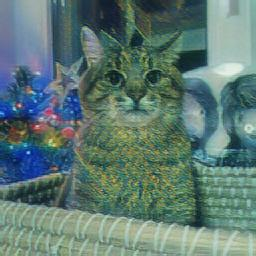
\includegraphics[scale=0.3]{./images/gen_5.jpg}
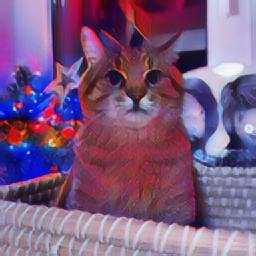
\includegraphics[scale=0.3]{./images/gen_6.jpg}
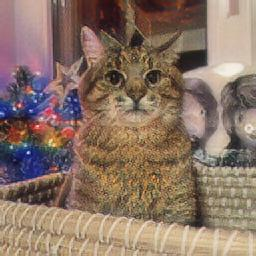
\includegraphics[scale=0.3]{./images/gen_7.jpg}
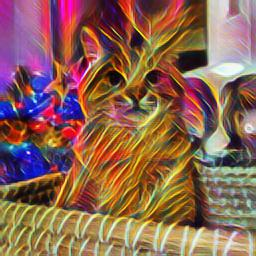
\includegraphics[scale=0.3]{./images/gen_9.jpg}
\end{frame}

\note{The seminal work of Gatys et al. demonstrated the power of Convolutional Neural Networks (CNNs) in creating artistic imagery by separating and recombining image content and style to obtain such paintings

}

\begin{frame}
\frametitle{A Neural Algorithm of Artistic Style \footfullcite{naas}}
    \begin{columns}
    	\column{0.5\textwidth}
       		\begin{figure}
   			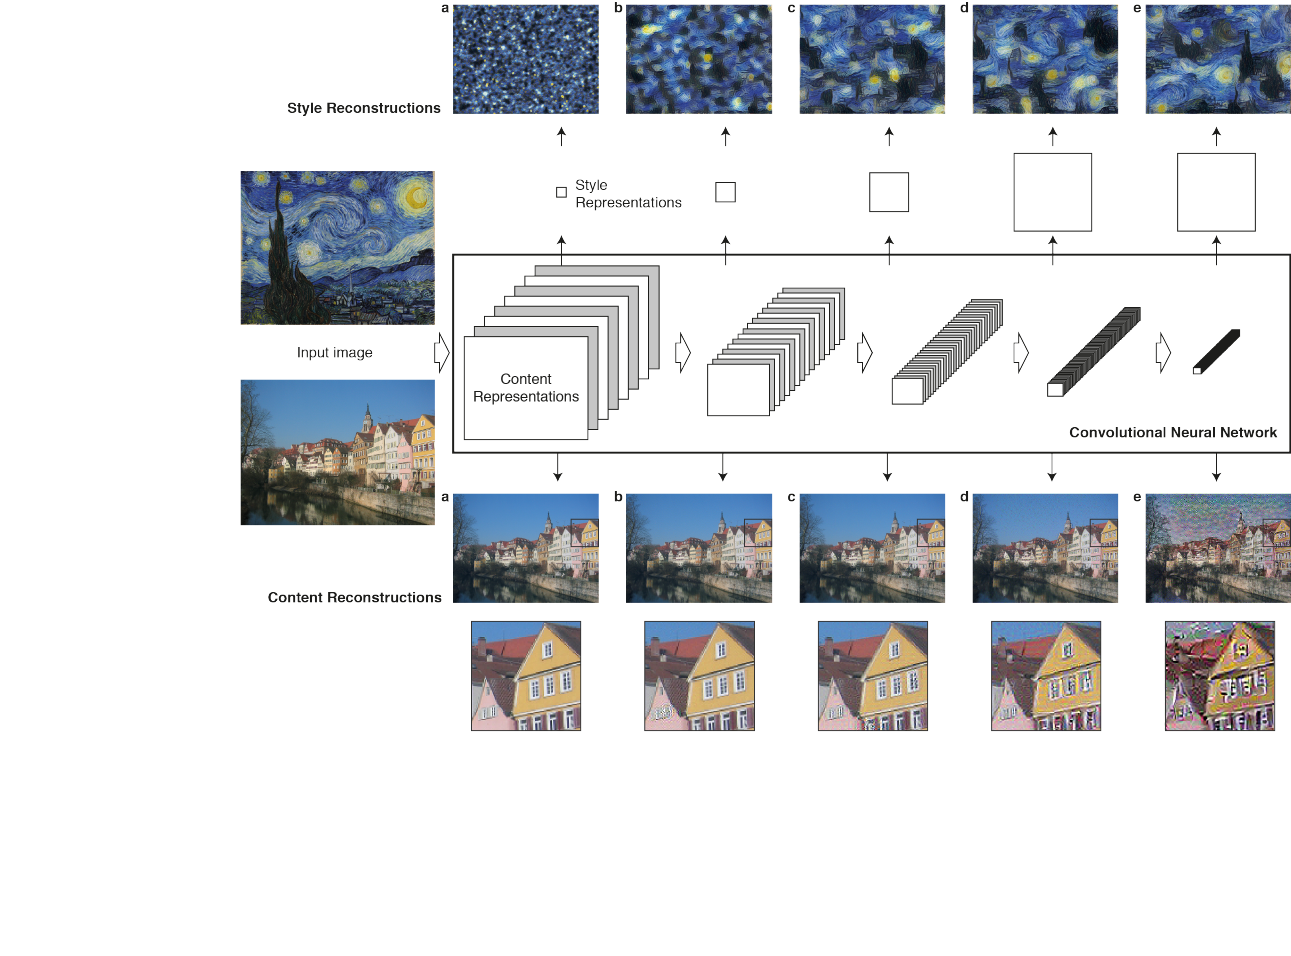
\includegraphics[scale=0.27]{network_model.png}
   		\end{figure}
	\column{0.5\textwidth}
	\begin{center}
	\vspace{-1cm}
	\begin{itemize}
	\item VGG16
	\item Style and content layers
	\end{itemize}
	\end{center}
\end{columns}
\vspace{-1cm}
		\begin{align*} \mathcal{L}_{tot} = \lambda_c \mathcal{L}_{c} +  \lambda_s \mathcal{L}_{s}  \text{ with : }&\mathcal{L}_{c} = \frac{1}{2}\sum_{i, j}\left(F_{ij}^l - P_{ij}^l\right)^2\\
		 &\mathcal{L}_{s} = \sum_{l=0}^L\left(w_l \frac{1}{4 N_l^2M_l^2}\sum_{i,j}\left(G_{ij}^l - A_{ij}^l\right)^2\right)
		\end{align*}
\end{frame}

\note{
{\tiny Recently, inspired by the power of Convolutional Neural Networks (CNNs), Gatys et al. [10] first studied how to use a CNN to reproduce famous painting styles on natural images. 

They proposed to model the content of a photo as the feature responses from a pre-trained CNN, and further model the style of an artwork as the summary feature statistics. 

Their experimental results demonstrated that a CNN is capable of extracting content information from an arbitrary photograph and style information from a well-known artwork. 

Based on this finding, Gatys et al. first proposed to exploit CNN feature activations to recombine the content of a given photo and the style of famous art-works. The key idea behind their algorithm is to iteratively optimise an image with the objective of matching desired CNN feature distributions, which involves both the photo’s content information and artwork’s style information. Their proposed algorithm successfully produces stylised images with the appearance of a given artwork.

The work of Gatys et al. opened up a new field called Neural Style Transfer (NST), which is the process of using Convolutional Neural Network to render a content image in different styles.

Higher layers in the network capture the high-level content in terms of objects and their arrangement in the input image but do not constrain the exact pixel values of the reconstruction. We therefore refer to these feature responses in higher layers of the network as the content representation.

To obtain a representation of the style of an input image, we use a feature space built on top of the filter responses in each layer of the network. By including the feature correlations of multiple layers, we obtain a stationary, multi-scale representation of the input image, which captures its texture information but not the global arrangement. We refer to this multi-scale representation as style representation.

The key finding of this paper is that the representations of content and style in the Convolutional Neural Network are separable. That is, we can manipulate both representations independently to produce new, perceptually meaningful images

}
}
\begin{frame}
    \frametitle{A Learned Representation For Artistic Style \footfullcite{lras}}
    	\begin{figure}
   		\centering
   		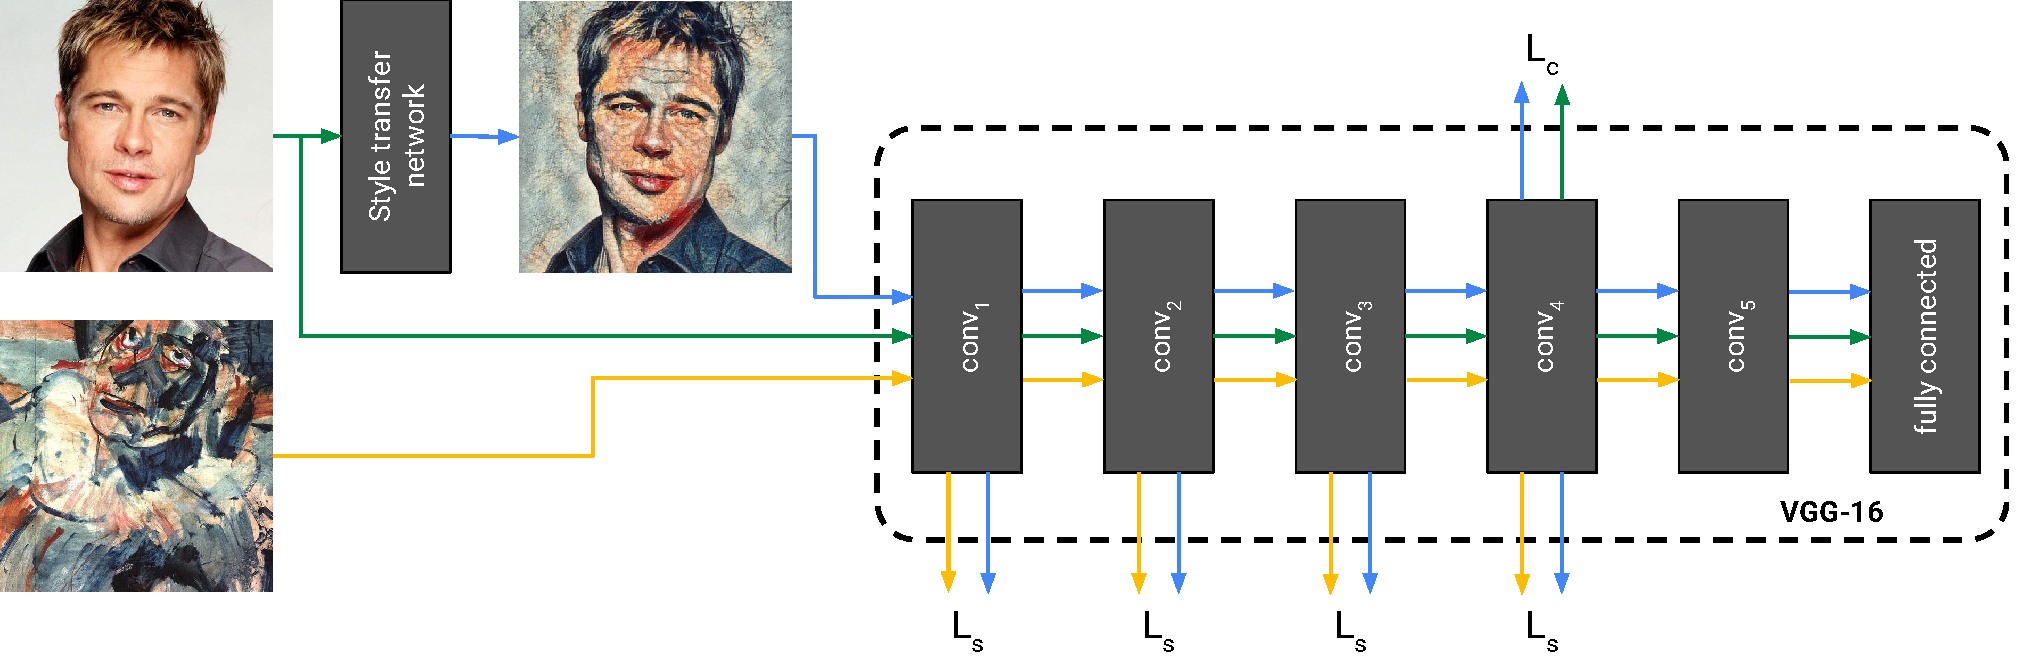
\includegraphics[scale=0.27]{style_transfer_network_diagram.pdf}
	\end{figure}
\begin{columns}
    	\column{0.5\textwidth}
       		$$ \mathcal{L}_{tot} = \lambda_c \mathcal{L}_{c}(T(c)) +  \lambda_s \mathcal{L}_{s}(T(c)) $$
	\column{0.5\textwidth}
	\begin{center}
	\begin{itemize}
		\item N-styles training
		\item Conditional Instance Normalization
	\end{itemize}
	\end{center}
\end{columns}
\end{frame}

\note{
{ \tiny While very flexible, this algorithm is expensive to run due to the optimization loop being carried. Ulyanov et al. (2016a), Li \& Wand (2016) and Johnson et al. (2016) tackle this problem by introducing a feedforward style transfer network, which is trained to go from content to pastiche image in one pass. However, in doing so some of the flexibility of the original algorithm is lost: the style transfer network is tied to a single style, which means that separate networks have to be trained for every style being modeled.
}
}

\begin{frame}
    \frametitle{LiveCam Style Transfer}
   	 \begin{itemize}
		\item \href{https://github.com/dabidou025/Live-Style-Transfer/}{GitHub}
	\end{itemize}
\end{frame}
\begin{frame}
\nocite{*}
\printbibliography
\end{frame}
\end{document}